\chapter{Experiment and Observation} \label{ch:experiment}

We obtained a digits dataset with 15 utterances per digit, and a commands (for the android project) dataset with 25 utterances per word. The recordings were done in moderately quiet environments using a general-purpose microphone.

\begin{figure}
    \centering
    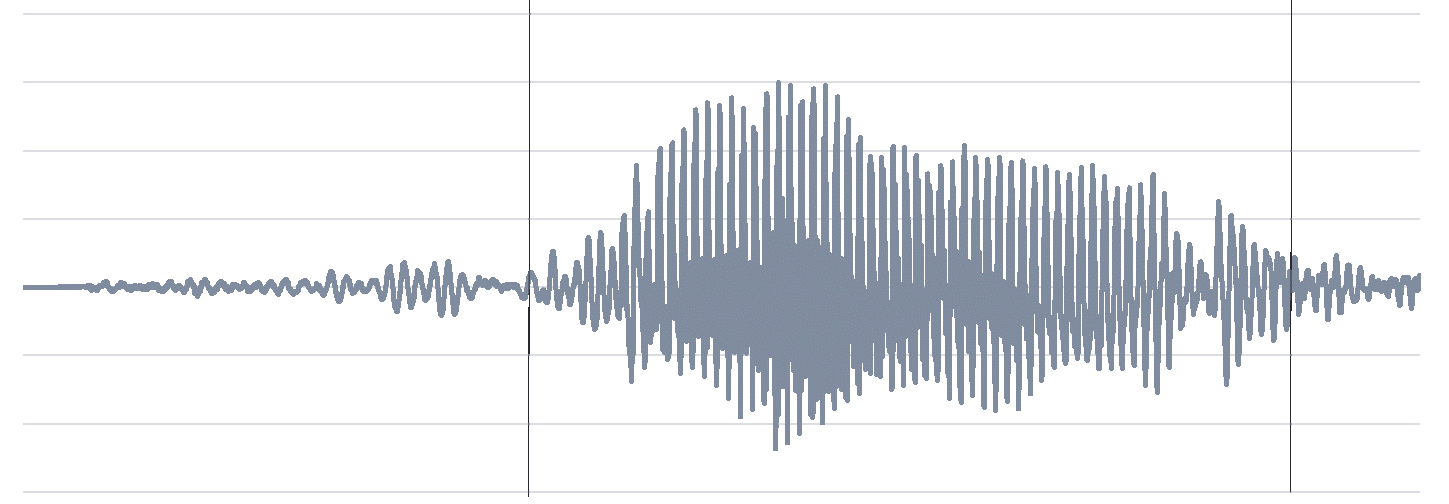
\includegraphics[scale=0.45]{graph-nine-trim}
    \label{fig:graph-nine-trim}
    \caption{Automatic trimming of nine}
\end{figure}

For the obtained datasets, the trimming algorithm presented very accurate results. The results were close to 88\% for the error of speech signal's endpoints missing by 100ms.

\newpage

\begin{figure}
    \centering
    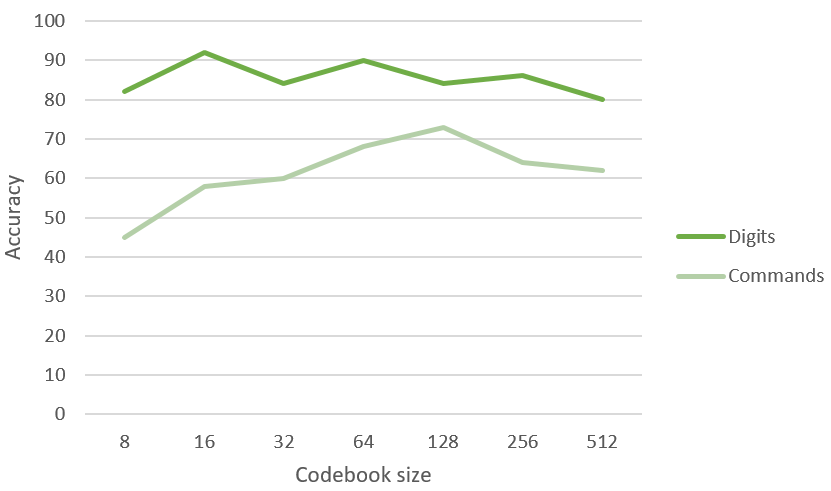
\includegraphics[scale=0.5]{graph-codebook-size}
    \label{fig:graph-codebook-size}
    \caption{Codebook size vs Accuracy}
\end{figure}

\begin{figure}
    \centering
    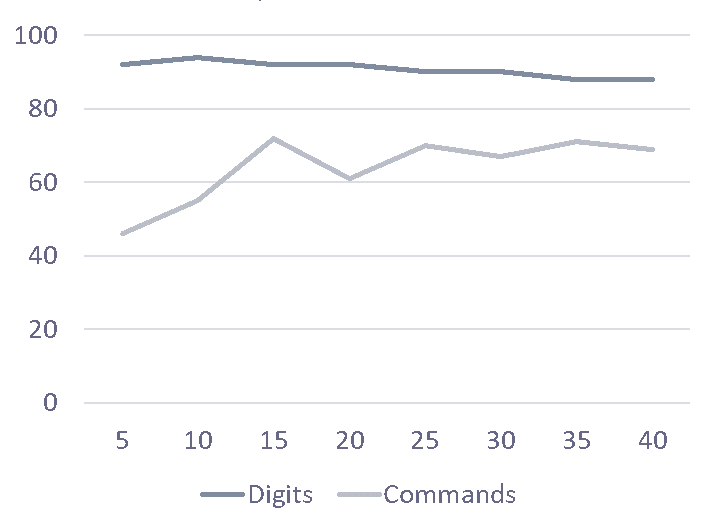
\includegraphics[scale=0.5]{graph-hidden-states}
    \label{fig:graph-hidden-states}
    \caption{Number of hidden states vs Accuracy}
\end{figure}

MFCC features resulted in better accuracy than LPCC features as expected. The accuracy of digits dataset decreased if delta or acceleration features were added, while it increased for commands dataset. The optimal codebook size and number of HMM states were higher for commands dataset than compared to digits dataset. Moreover, initial Bakis model with more jumps improved the performance for commands dataset.

\hfill

\begin{table}[H]
    \centering
    \begin{tabular}{lll}
    \hline
    Description           & Digits dataset & Commands dataset \\
    \hline
    Number of words       &  10     & 21 \\
    Number of utterances  &  150    & 525 \\
    \hline
    Delta features        &  No     & Yes \\
    Delta delta feautres  &  No     & Yes \\
    Codebook size         &  16  & 128 \\
    Number of hidden states  &  10 & 15 \\
    Jumps allowed in Bakis &  1 & 3 \\
    \hline
    Training time (s)     &  3.3 & 7.4 \\
    Accuracy (\%)         &  94 & 73 \\
    \hline
    \end{tabular}
    \caption{Results of speech recognition}
\end{table}   

For profiling the library on a desktop, Visual Studio Profiler was used and a Intel Corei7 3.0GHz + 8GB RAM laptop was selected. During training, the maximum CPU usage increased up to 80\% while the maximum RAM usage was below 20MB for our datasets.

For profiling the android application, Android Studio Profiler was used and an octa-core 1.7GHz + 2GB RAM mobile phone was selected. During testing, the maximum CPU usage increased up to 50\% while the RAM stayed constant at 12MB. The average recognition time for input utterances was 15ms.

It was observed that the system was not accurate enough for speaker independent scenarios with accuracy as low as 40\%. Noisy environments, changes in pitch and accents, similar sounding words in the dataset, and improper training parameters also reduced the accuracy of the system.